% Antecedentes
\begin{frame}
  \frametitle{Antecedentes I.}    
  Sea $P$ un polígono simple con $n$ vértices. Definimos
  \begin{itemize}
  \item $int(P) \rightarrow \#$ aristas estrictamente internas. 
  \item $ext(P) \rightarrow \#$ aristas estrictamente externas.
  \item Vértice interno de $P$ si pertenece al interior de $Conv(P)$.
  \end{itemize}
    \begin{figure}
    \centering
    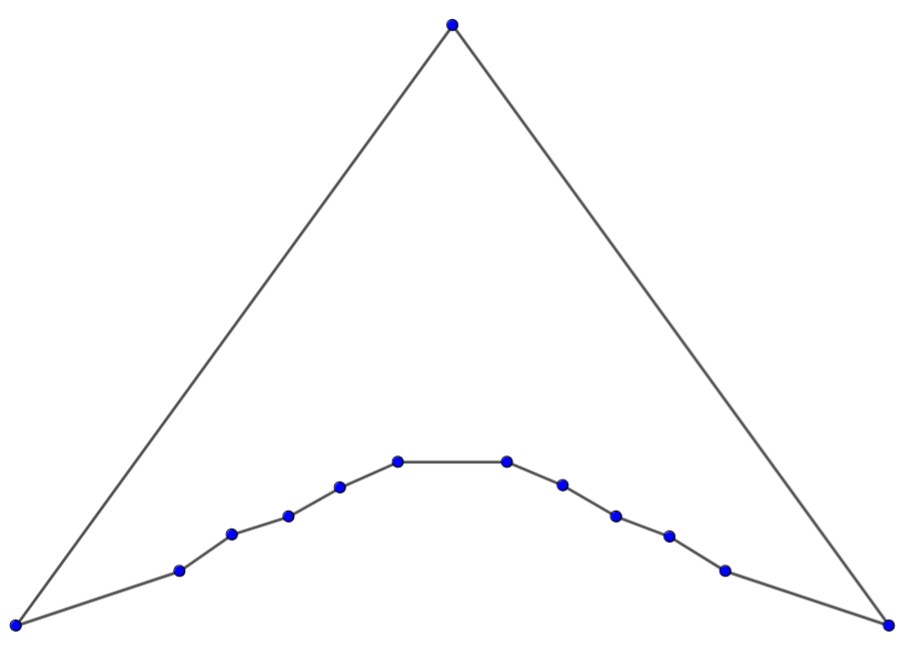
\includegraphics[width=.30 \paperwidth]{./images/Ejemplo1.png}
    \caption*{Polígono.}
  \end{figure}
\end{frame}


\begin{frame}
  \frametitle{Antecedentes I.}    
  Sea $P$ un polígono simple con $n$ vértices. Definimos
  \begin{itemize}
  \item $int(P) \rightarrow \#$ aristas estrictamente internas. 
  \item $ext(P) \rightarrow \#$ aristas estrictamente externas.
  \end{itemize}
    \begin{figure}
    \centering
    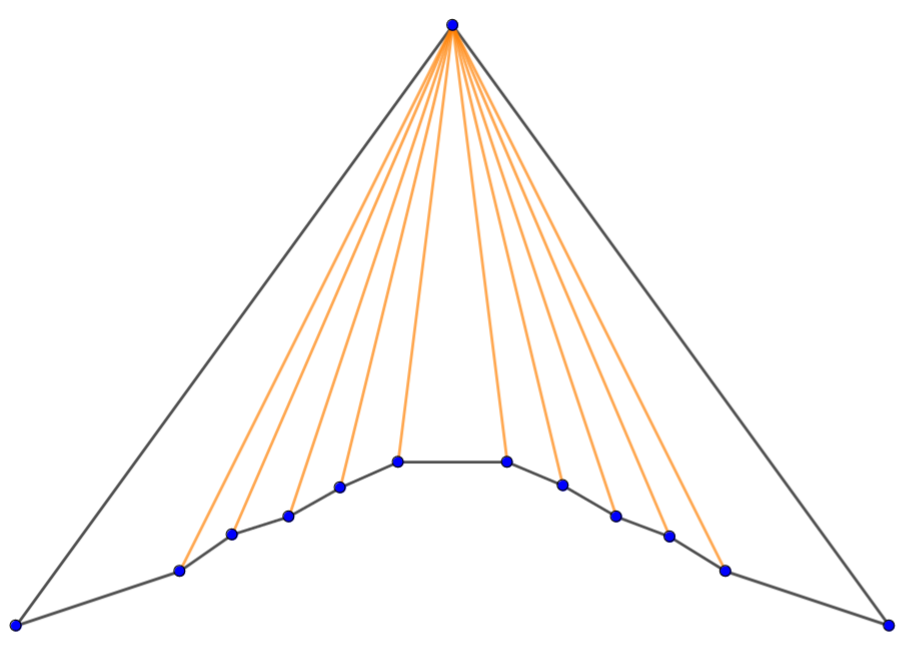
\includegraphics[width=.35 \paperwidth]{./images/Ejemplo2.png}
    \caption*{Algunas aristas extrictamente internas.}
  \end{figure}
\end{frame}

\begin{frame}
  \frametitle{Antecedentes I.}    
  Sea $P$ un polígono simple con $n$ vértices. Definimos
  \begin{itemize}
  \item $int(P) \rightarrow \#$ aristas estrictamente internas. 
  \item $ext(P) \rightarrow \#$ aristas estrictamente externas.
  \end{itemize}
  \begin{figure}
    \centering
    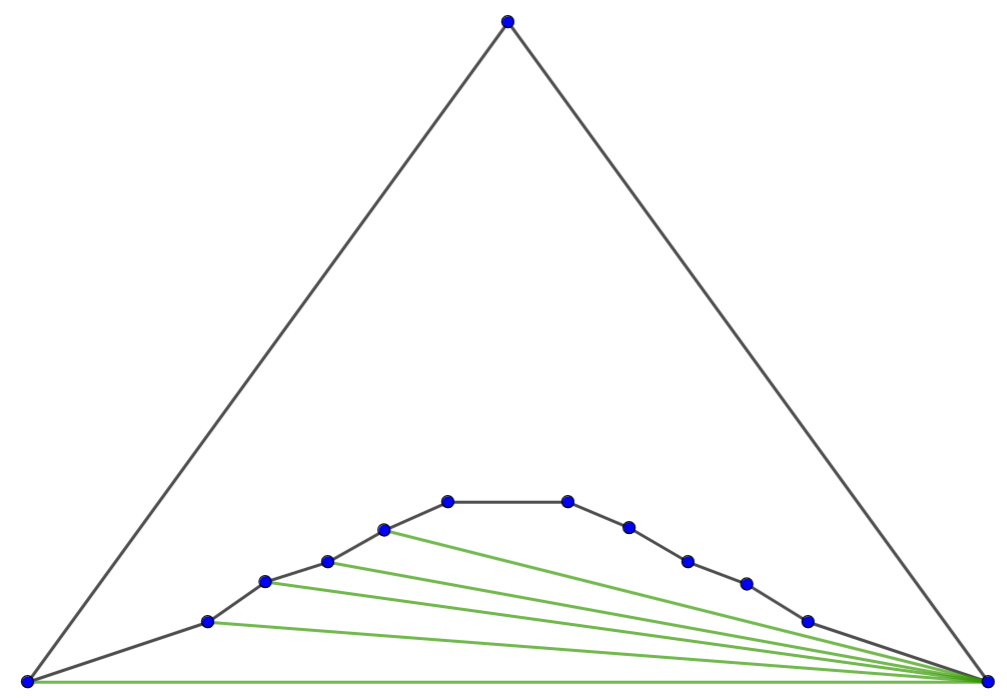
\includegraphics[width=.35 \paperwidth]{./images/Ejemplo3.png}
    \caption*{Algunas aristas extrictamente externas.}
  \end{figure}
\end{frame}

\begin{frame}
  \frametitle{Antecedentes II.}    
  \begin{lema}
    Sea $P$ un polígono de $n$ vértices, con $k$ vértices internos. Entonces \[ext(P) \geq k.\]
  \end{lema}
  \textbf{Dem.} Analicemos dos posibles casos:\newline
  \textit{Caso 1.} $p \in V_P$ tal que es interno y sus vecinos son parte de $V_{Conv(P)}$. Entonces
  existe una $e \in E_{Conv(P)}$ que es estrictamente externa.
  \begin{figure}
    \centering
    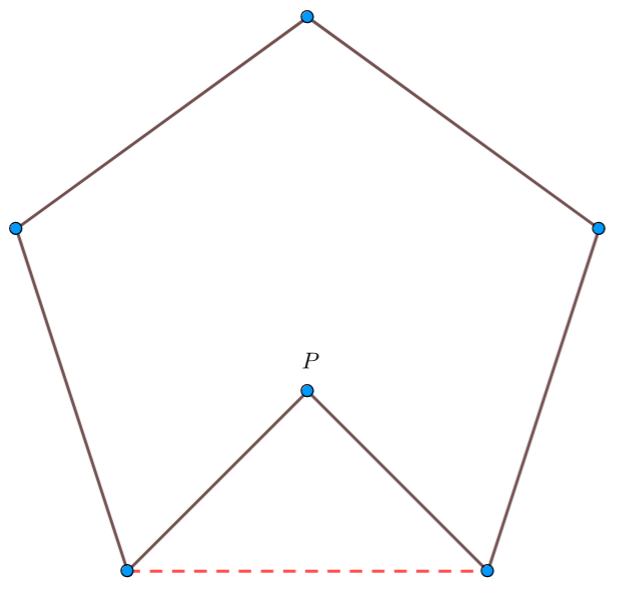
\includegraphics[width=.15 \paperwidth]{./images/Caso01.png}
    %\caption*{Caso 1.}
  \end{figure}
\end{frame}

\begin{frame}
  \frametitle{Antecedentes II.}    
  \begin{lema}
    Sea $P$ un polígono de $n$ vértices, con $k$ vértices internos. Entonces \[ext(P) \geq k.\]
  \end{lema}
  \textbf{Dem.} Analicemos dos posibles casos:\newline
  \textit{Caso 2.} Hay al menos $2$ vértices vecinos internos. Entonces hay una arista extrictamente externa
  y al menos tantas extrictamente externas cómo vértices internos en esta sección.
  \begin{figure}
    \centering
    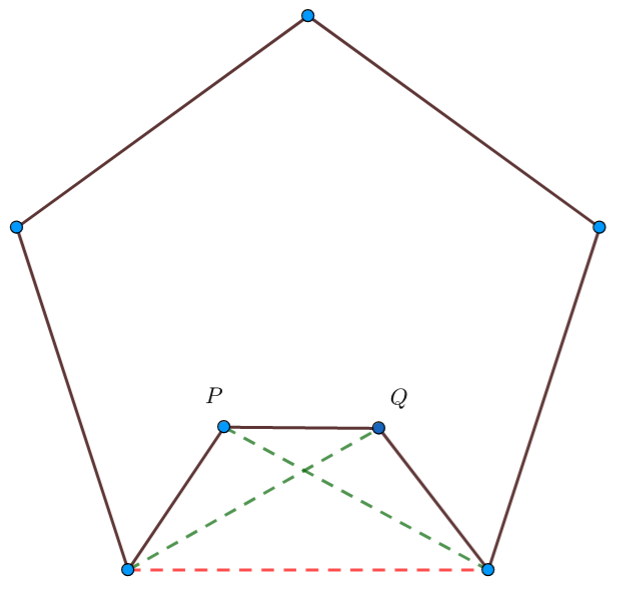
\includegraphics[width=.15 \paperwidth]{./images/Caso02.png}
    %\caption*{Caso 1.}
  \end{figure}
  \hfill $\square$\newline
  
  .\newline

  .
\end{frame}

\begin{frame}
  \frametitle{Antecedentes III.}    
  \begin{lema}
    Si $P$ tiene $k$ vértices internos, entonces \[int(P) + ext(P) \geq (n + 3) + k.\]
  \end{lema}
  \textbf{Dem.} $int(P) = n - 3$. Entonces
  \begin{eqnarray*}
    int(P) &\geq& n - 3\\
    ext(P) &\geq& k\\
    \Rightarrow int(P) + ext(P) &\geq& (n + 3) + k.
  \end{eqnarray*}
  De lo anterior terminamos. \hfill $\square$
\end{frame}

\begin{frame}
  \frametitle{Antecedentes IV.}    
  \begin{lema}
    Todo polígono con $k$ vértices internos puede descomponerse en $k + 1$ polígonos
    convexos $P_1, \dotsm, P_{k + 1}$. Esta descomposición puede obtenerse de tal forma
    que si $P_i$ tiene $n_i$ vértices $i \in [1, \dotsm, k+1]$ entonces $n_1 + \dotsm + n_{k + 1} = n + 3k$.
  \end{lema}
  \textbf{Dem.} Para cada uno de los vértices internos $v$ de $P$, dibújese un
  segmento de lıínea que bisecte el ángulo interno de $P$ en $v$, y que se extiende hasta
  intersectar una arista de $P$ o un bisector previamente dibujado.\newline
\end{frame}

\begin{frame}
  \frametitle{Antecedentes IV.}    
  \begin{figure}
    \centering
    \includegraphics[width=.35 \paperwidth]{./images/Polígono.png}
    \caption*{División de un polígono.}
  \end{figure}
  Observemos que cada vértice interno de $P$ aparece en exactamente dos
  subpolıígonos convexos de $P$ , y que los extremos finales de nuestros bisectores
  también aparecen dos veces en esos polıígonos. \hfill $\square$
\end{frame}

\begin{frame}
  \frametitle{Antecedentes V.}
  \begin{lema}
    Sea $P_i'$ el polígno formado por vértices reales para cada $P_i$ y sea $m_i$ el número
    de vértices de $P_i'$. Entonces si $m_i \geq 4$, entonces cualquier arista extrictamente
    interna de $P_i$ es intersectada por, al menos, $m_i - 3$ aristas estrictamente internas
    de $P_i'$.
  \end{lema}
  \textbf{Dem.} Por el hecho de triangular. $P_i$ es el polígono resultante del lema anterior
  y $P_i'$ es formado a partir de los vértices reales de este, entonces $m_i = |V_{P_i'}|$.
  \hfill $\square$
\end{frame}
